\documentclass[twoside]{article}
\usepackage{amsgen,amsmath,amstext,amsbsy,amsopn,amssymb,}
\usepackage{graphicx}
\usepackage{epsfig}

\setlength{\oddsidemargin}{0.1 in} \setlength{\evensidemargin}{-0.1
in} \setlength{\topmargin}{-1 in} \setlength{\textwidth}{6.5 in}
\setlength{\textheight}{10.5 in} \setlength{\headsep}{0.1 in}
\setlength{\parindent}{0 in} \setlength{\parskip}{0.1 in}

\newcommand{\homework}[2]{
   \pagestyle{myheadings}
   \thispagestyle{plain}
   \newpage
   \setcounter{page}{1}
   \noindent
   \begin{center}
   \framebox{
      \vbox{\vspace{2mm}
       \hbox to 6.28in { {\bf Math 1700:~Elementary Statistics \hfill} }
       \vspace{6mm}
       \hbox to 6.28in { {\Large \hfill #1 (#2)  \hfill} }
       \vspace{6mm}
      \vspace{2mm}}
   }
   \end{center}
   \markboth{#1}{#1}
   \vspace*{4mm}
}

\newcommand{\bbF}{\mathbb{F}}
\newcommand{\bbX}{\mathbb{X}}
\newcommand{\bI}{\mathbf{I}}
\newcommand{\bX}{\mathbf{X}}
\newcommand{\bY}{\mathbf{Y}}
\newcommand{\bepsilon}{\boldsymbol{\epsilon}}
\newcommand{\balpha}{\boldsymbol{\alpha}}
\newcommand{\bbeta}{\boldsymbol{\beta}}
\newcommand{\0}{\mathbf{0}}

\begin{document}

\homework{$2^{nd}$ Week Summary}{09/04/25}
\begin{itemize}

\vspace{-.25in}
\begin{figure}[h]
\hspace{5in}
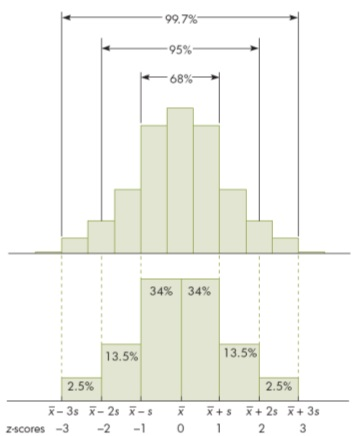
\includegraphics[angle=0,width=2in] {graphs2-0.jpg}
\end{figure}

\vspace{-2.75in}
\begin{figure}[h]
\hspace{3.25in}
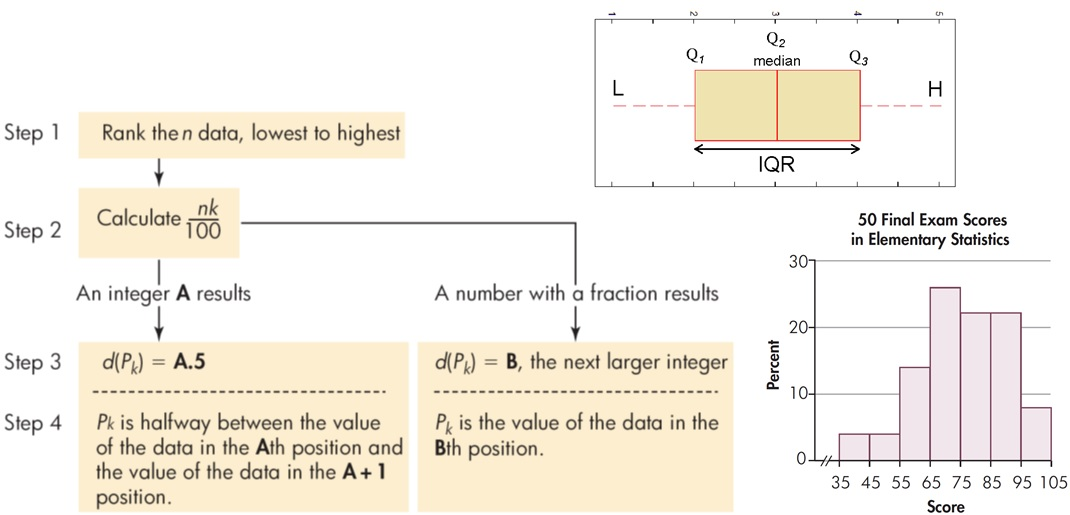
\includegraphics[angle=0,width=2in] {graphs2.jpg}
\end{figure}

\vspace{-1.2in}
\item Measures of Position
\subitem Quartiles: $Q_1, Q_2 (\tilde{x}), Q_3$
\subitem Percentile: $P_k$
\subitem Five number summary: $(L, Q_1, Q_2, Q_3, H)$
\subitem Interquartile range: $IQR=Q_3-Q_1$
\item Box-and-whiskers display
\item Standard score, or z-score
\subitem $z_i=\dfrac{x_i-\bar{x}}{s}$
\item Empirical Rule ($68-95-99.7$ Rule)
\item Comparing the measures of center and spread

\item \textbf{Bivariate Data:}
\item Qualitative vs Qualitative
\subitem Contingency table
\item Qualitative vs Quantitative
\subitem Side-by-side Box Plot
\item Quantitative vs Quantitative
\subitem Scatter diagram

\vspace{-3in}
\begin{figure}[h]
\hspace{3.2in}
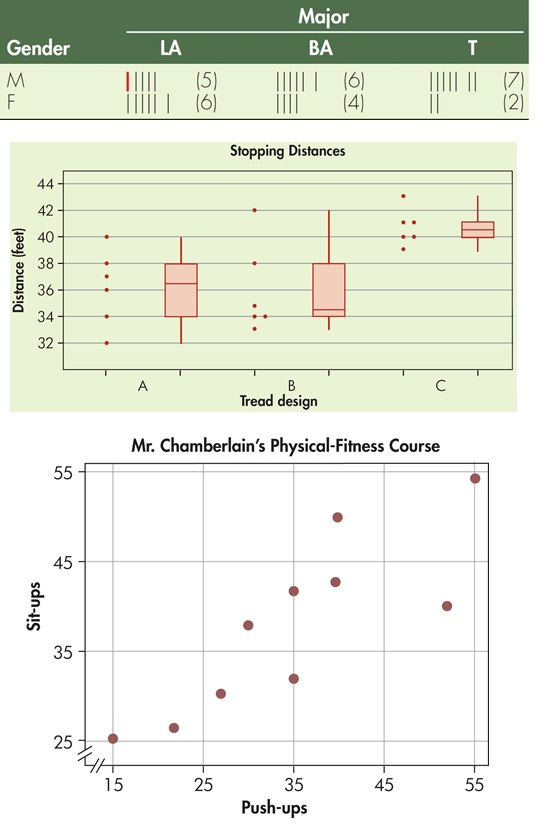
\includegraphics[angle=0,width=1.75in] {graphs3-0.jpg}\\
\begin{center}
\hspace{3.4in}
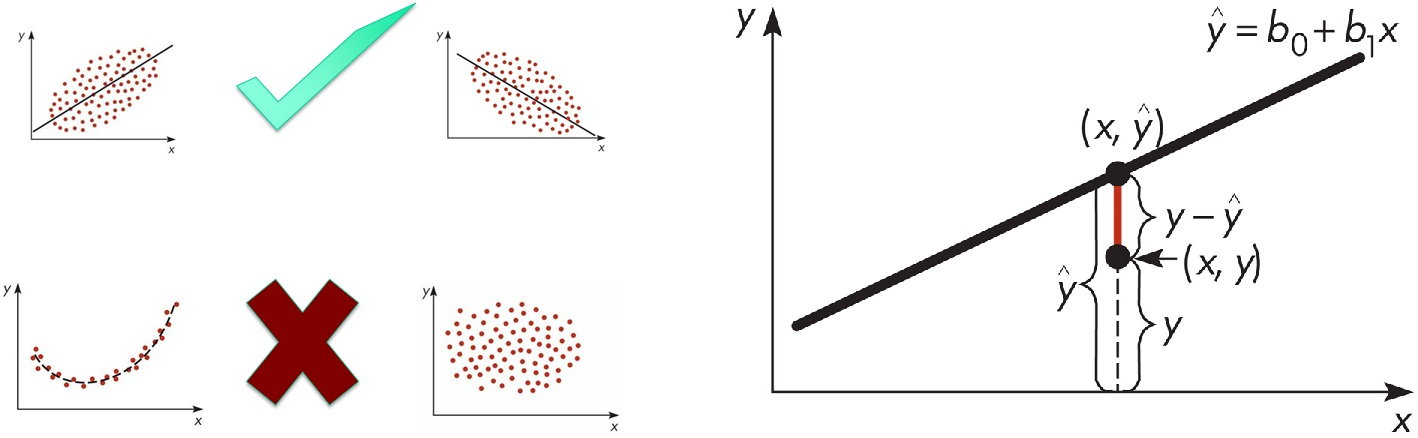
\includegraphics[angle=0,width=3in] {graphs3.jpg}
\end{center}
\end{figure}

\vspace{-1.2in}
\item \textbf{Linear Correlation:} $r=\dfrac{SS(xy)}{\sqrt{SS(x)SS(y)}}$, where
\subitem $SS(x)=\sum_{i=1}^nx_i^2-\dfrac{1}{n}\left(\sum_{i=1}^nx_i\right)^2$
\subitem $SS(y)=\sum_{i=1}^ny_i^2-\dfrac{1}{n}\left(\sum_{i=1}^ny_i\right)^2$
\subitem $SS(xy)=\sum_{i=1}^nx_iy_i-\dfrac{1}{n}\left(\sum_{i=1}^nx_i\right)\left(\sum_{i=1}^ny_i\right)$
\item Properties of the Correlation r:
\subitem Takes values between $-1$ and $1$
\subitem $r = 1$ or $r = -1$ implies that the points lie on a straight line
\subitem $r = 0$ implies that there is no \textbf{linear} association
\subitem $r < 0$ implies that there is a negative \textbf{linear} association \& $r > 0$ implies positive \textbf{linear} association
\subitem $r$ is strongly affected by a few outliers

\item \textbf{Linear Regression:} $\hat{y}=b_0+b_1x$
\subitem where, $\hat{y}$ represents the predicted value of $y$ that corresponds to a particular value of $x$
\item The Least Squares Criterion: Finding $b_0$ and $b_1$ such that $\sum_{i=1}^n(y_i-\hat{y}_i)^2$ is as small as possible
\subitem The slope: $b_1=\dfrac{SS(xy)}{SS(x)}$, represents the predicted change in $y$ per unit increase in $x$
\subitem The $y$-intercept: $b_0=\bar{y}-b_1\bar{x}$, is the value of $y$ \ where the line of best fit intersects the $y$-axis
\item \textbf{Causation and Lurking Variable:}
\subitem Simpson’s Paradox
\end{itemize}
\end{document}
